\documentclass[10pt]{article}
\usepackage{geometry}                % See geometry.pdf to learn the layout options. There are lots.
\geometry{a4paper
}                   % ... or a4paper or a5paper or ... 
\usepackage[parfill]{parskip}    % Activate to begin paragraphs with an empty line rather than an indent

%%%%%%%%%%%%%%%%%%%%
\newcommand{\hide}[1]{}

\usepackage{natbib}
\usepackage{xcolor}
\usepackage{url}
\usepackage{hyperref}
\usepackage{mathtools}
\usepackage{array}
\usepackage{multirow}
\usepackage{graphicx}
\usepackage{subcaption}
\usepackage{mwe}
\usepackage{float}
\usepackage{tikz}

\hide{
\usepackage{amscd}
\usepackage{amsfonts}
\usepackage{amsmath}
\usepackage{amssymb}
\usepackage{amsthm}
\usepackage{cases}		 
\usepackage{cutwin}
\usepackage{enumerate}
\usepackage{epstopdf}
\usepackage{graphicx}
\usepackage{ifthen}
\usepackage{lipsum}
\usepackage{mathrsfs}	
\usepackage{multimedia}
\usepackage{wrapfig}
}

	 
%\input{/usr/local/LATEX/Lee_newcommands.tex}
\newcommand{\itemlist}[1]{\begin{itemize}#1\end{itemize}}
\newcommand{\enumlist}[1]{\begin{enumerate}#1\end{enumerate}}
\newcommand{\desclist}[1]{\begin{description}#1\end{description}}

\newcommand{\Answer}[1]{\begin{quote}{\color{blue}#1}\end{quote}}
\newcommand{\AND}{\wedge}
\newcommand{\OR}{\vee}
\newcommand{\ra}{\rightarrow}
\newcommand{\lra}{\leftrightarrow}

\newcommand\MyBox[1]{%
  \fbox{\parbox[c][.7cm][c]{.7cm}{\centering #1}}%
}
\newcommand\MyVBox[1]{%
  \parbox[c][.7cm][c]{1cm}{\centering\bfseries #1}%
}
\newcommand\MyHBox[2][\dimexpr.7cm+2\fboxsep\relax]{%
  \parbox[c][1cm][c]{#1}{\centering\bfseries #2}%
}
\usepackage{etoolbox}
\newcommand\MyTBox[2]{%
  \MyVBox{#1}
  \renewcommand*\do[1]{\MyBox{##1}\hspace*{-\fboxrule}}
  \docsvlist{#2}
  \par\vspace{-\fboxrule}
}

\title {CS36110 Machine Learning Assignment}


\date{}                                           % Activate to display a given date or no date

\begin{document}
\maketitle

\section*{Task 1}

\subsection*{Part A}
The first algorithm I used was the J48 Decision Tree classifier this is an implementation of the ID3 algorithm with Rule Post-Pruning. ID3 grows a decision tree recursively where at each node it selects the feature with the highest information gain that best classifies the training data it was given, when the tree is grown Rule Post-Pruning (RPP) is then run over the entire tree. RPP converts each path through the tree to a rule and then independently evaluates each rule to see if it affects the validation accuracy of the tree and if it doesn't then it is pruned out. J48 mitigates overfiting because it uses RPP this helps the algorithm make a decision tree that more accurately fits the patterns in the data instead of fitting to the data itself.

The second classifier I used was Naive Bayes and it works by calculating the probabilities of events occurring within the data set it does this using Bayes Theorem which is shown in Figure \ref{fig:bayes} and works be relating the Posterior Probability $(P(A \mid B))$ with the prior probability of the hypothesis $(P(A))$ and the conditional probability of the data under the hypothesis $(P(B \mid A))$. To classify a new piece of data you work out the probability for each decision class using the training data and the class with the highest probability is the one that you assign that data to. Naive Bayes doesn't go through a long training sequence so this makes it very fast when you want to classify a piece of data, this also makes it quick and easy to update when you get new training data.

An advantage J48 has over Naive Bayes is that Naive Bayes assumes that all the data is independent which isn't true in real life applications this can result in a poor accuracy of the trained model.


\begin{figure}[h]
    \centering
    $$ P(A \mid B) = \frac{P(B \mid A) \, P(A)}{P(B)} $$
    \caption{Bayes Theorem.}
    \label{fig:bayes}
\end{figure}

\newpage
\subsection*{Part B}
Over the entire training data set the J48 model obtained a recall measurement of 71.9\% compared to Naive Bayes 55.7\%, recall is a measure of of the ratio of the number of correct positive examples out of those which were classified as positive\cite{MarslandStephen2015Ml:a} a higher recall measure means that more instances are being correctly classified. Precision is the ratio of correct positive examples to the number of actual positive examples\cite{MarslandStephen2015Ml:a}, the precision for J48 is 71.8\% and for Naive Bayes it is 58.7\% the higher precision means that the classifier successfully classified more results. 

A measure you could use is the Receiver Operator Characteristic Curve this is a plot of false positive rate along the x axis and true positive rate along the y axis, a perfect classifier would be a plot at (0,1) which would mean 100\% true positives and 0\% false positives. Figures \ref{fig:naive bayes roc curves} and \ref{fig:c45 roc curves} show these ROC curves and their Area Under Curve (AUC). The ROC curve is not useful in this context because it's not meant for multi class problems, in general it is useful for two class problems because the area under the curve represents how well the classifier differentiates between two classes.

Figures \ref{fig:j48 confusion matrix} and \ref{fig:nb confusion matrix} below show the confusion matrices for the J48 classifier and the Naive Bayes classifier, from these matrices you can see how well the classifiers perform. You can clearly see how much better the J48 classifier is compared to Naive Bayes, if you look at the leading diagonal for J48 then you can see how much better it is. If you look at class C for Naive Bayes this inaccuracy really shows because only 49 instances where correctly classified with the majority being incorrectly classified as B this is an accuracy of only 29\%. 

%J48 confusion Matrix
\begin{figure*}[h]
    \centering
    {
    \offinterlineskip
    \hspace*{1cm}\MyHBox{A}\MyHBox{B}\MyHBox{C}
    \MyHBox{D}\par
    
    \MyTBox{A}{107, 20, 11, 14}
    \MyTBox{B}{23, 103, 20, 13}
    \MyTBox{C}{13, 24, 110,  21}
    \MyTBox{D}{9,  11,  11, 167}
    }
    \caption{The confusion matrix for the J48 decision tree classifier.}
    \label{fig:j48 confusion matrix}
\end{figure*}

%NB confusion Matrix
\begin{figure*}[h]
    \centering
    {
    \offinterlineskip
    \hspace*{1cm}\MyHBox{A}\MyHBox{B}\MyHBox{C}
    \MyHBox{D}\par
    
    \MyTBox{A}{90,  27,  10,  25}
    \MyTBox{B}{40,  98,  10,  11}
    \MyTBox{C}{40,  58,  49,  21}
    \MyTBox{D}{27,  27,   4, 140}
    }
    \caption{The confusion matrix for the Naive Bayes classifier.}
    \label{fig:nb confusion matrix}
\end{figure*}

The Kappa statistic compares an observed accuracy with an expected accuracy and is useful in evaluating classifiers because it takes into account the random chance this makes it generally less misleading than accuracy. The Kappa statistic for Naive Bayes is 0.4091 and for J48 it is 0.6239, There is not a standardized interpretation of this statistic but Landis and Koch\cite{landiskochkappa} consider 0-0.20 as slight, 0.21-0.40 as fair, 0.41-0.60 as moderate, 0.61-0.80 as substantial, and 0.81-1 as almost perfect. Under this Naive Bayes would be classified as moderate and J48 as substantial. 

\begin{figure*}[h]
    \centering
    \begin{subfigure}[b]{0.475\textwidth}
        \centering
        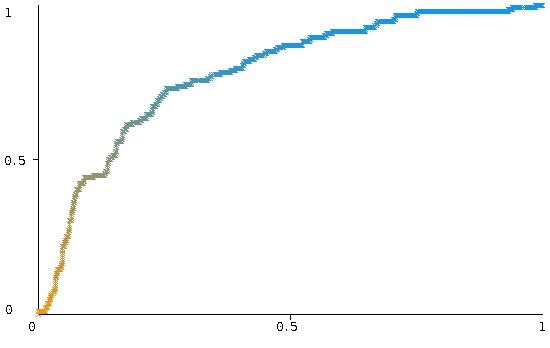
\includegraphics[width=\textwidth]{bayes_roc/roc_curve_a.jpg}
        \caption[Network2]%
        {{\small The ROC for class a, the area under ROC is 0.7803.}}    
        \label{fig:bayes roc curve class a}
    \end{subfigure}
    \hfill
    \begin{subfigure}[b]{0.475\textwidth}  
        \centering 
        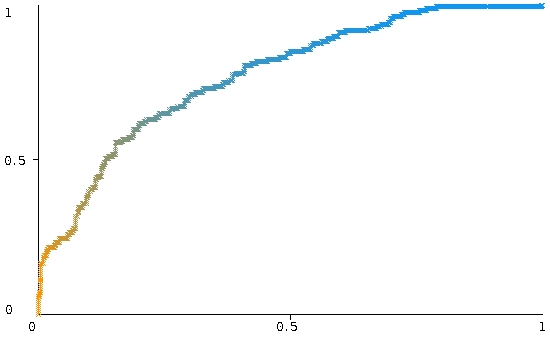
\includegraphics[width=\textwidth]{bayes_roc/roc_curve_b.jpg}
        \caption[]%
        {{\small The ROC for class b, the area under ROC is 0.7723.}}    
        \label{fig:bayes roc curve class b}
    \end{subfigure}
    \vskip\baselineskip
    \begin{subfigure}[b]{0.475\textwidth}   
        \centering 
        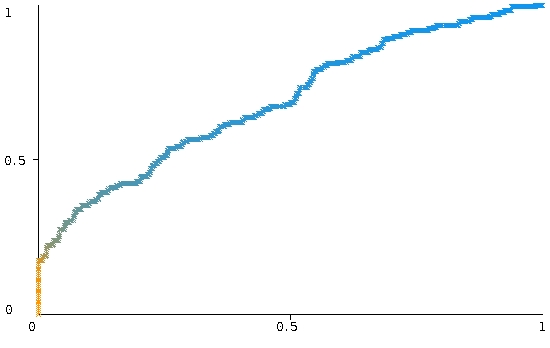
\includegraphics[width=\textwidth]{bayes_roc/roc_curve_c.jpg}
        \caption[]%
        {{\small The ROC for class c, the area under ROC is 0.6881.}}    
        \label{fig:bayes roc curve class c}
    \end{subfigure}
    \quad
    \begin{subfigure}[b]{0.475\textwidth}   
        \centering 
        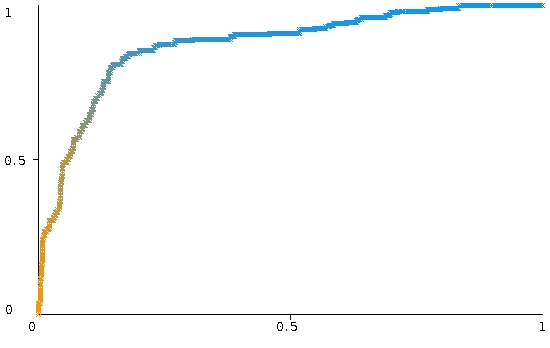
\includegraphics[width=\textwidth]{bayes_roc/roc_curve_e(d).jpg}
        \caption[]%
        {{\small The ROC for class d, the area under ROC is 0.8715.}}    
        \label{fig:bayes roc curve class d}
    \end{subfigure}
    \caption[ ]
    {\small The Receiver Operator Characteristic Curve for the Naive Bayes classifier} 
    \label{fig:naive bayes roc curves}
\end{figure*}

\begin{figure*}[h]
    \centering
    \begin{subfigure}[b]{0.475\textwidth}
        \centering
        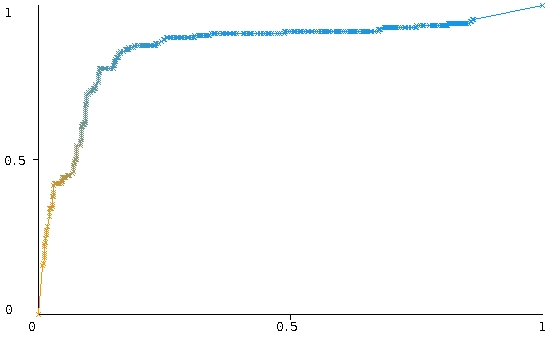
\includegraphics[width=\textwidth]{c45_roc/roc_curve_a.jpg}
        \caption[Network2]%
        {{\small The ROC for class a, the area under ROC is 0.8613.}}    
        \label{fig:c45 roc curve class a}
    \end{subfigure}
    \hfill
    \begin{subfigure}[b]{0.475\textwidth}  
        \centering 
        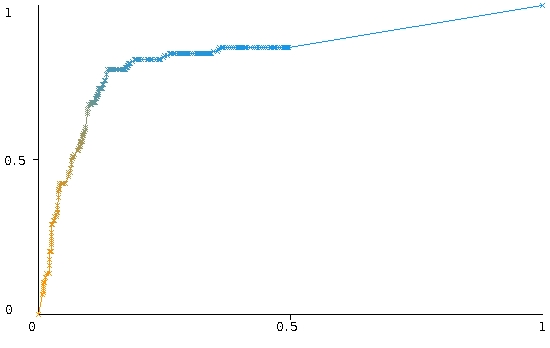
\includegraphics[width=\textwidth]{c45_roc/roc_curve_b.jpg}
        \caption[]%
        {{\small The ROC for class b, the area under ROC is 0.8341.}}    
        \label{fig:c45 roc curve class b}
    \end{subfigure}
    \vskip\baselineskip
    \begin{subfigure}[b]{0.475\textwidth}   
        \centering 
        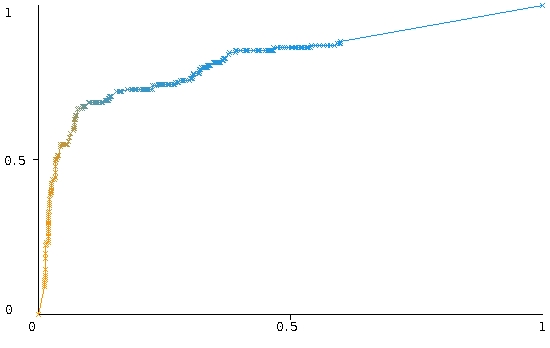
\includegraphics[width=\textwidth]{c45_roc/roc_curve_c.jpg}
        \caption[]%
        {{\small The ROC for class c, the area under ROC is 0.8208.}}    
        \label{fig:c45 roc curve class c}
    \end{subfigure}
    \quad
    \begin{subfigure}[b]{0.475\textwidth}   
        \centering 
        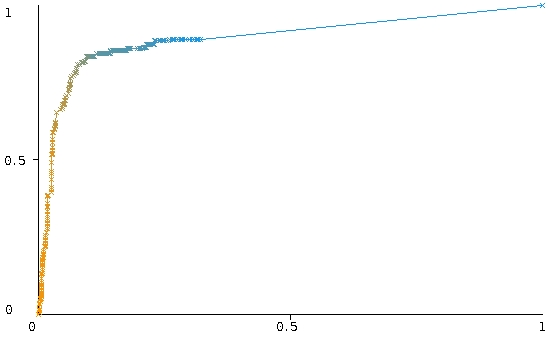
\includegraphics[width=\textwidth]{c45_roc/roc_curve_e(d).jpg}
        \caption[]%
        {{\small The ROC for class d, the area under ROC is 0.892.}}    
        \label{fig:c45 roc curve class d}
    \end{subfigure}
    \caption[ ]
    {\small The Receiver Operator Characteristic Curve for the J48 Classifier} 
    \label{fig:c45 roc curves}
\end{figure*}



\subsection*{Part C}
% A baseline classifier is something that provides a prediction in a very simple way, Weka includes a baseline classifier called ZeroR which works by predicting a majority class this achieved 29.25\% accuracy which shows that the classifiers I chose previously have massively outperformed this and they are much better than the baseline.

I think randomness would be a good baseline to test against, a classifier that randomly chooses one of the four absence classes. If you used this over a dataset that had an equal number of instances from each class then you would expect an accuracy of around 25\%. This would be a good baseline because it's very easy to implement and would be very fast to run and test.

\section*{Task 2}

\subsection*{Part A}
There are a few different ways of handling missing values. You could remove the missing values entirely so that data is no longer in the set or you could work out the average value for the missing data and use that. This is what Wekas implementation of Naive Bayes does if there are missing values then before it runs it will populate those values with the mean from the dataset, however sometimes this approach isn't very meaningful because for binary features the mean could be somewhere in the middle and then you have to somehow interpret that. You could use probability theory to look at the distributions and then take the missing value from that.

There is a filter in Weka called RepalceMissingValues this filter replaces all missing values  with the modes and means from the training data. When replacing missing values with the mean you can bias your dataset, to avoid this you should consider the mean and mode of all the instances from the training data rather than just from the class. If this approach was followed then you would only see an increase for the Naive Bayes classifier because this approach is what J48 does when it encounters missing data.

Another filter is the RemoveWithValues filter this allows you to filter and match certain pieces of data and then remove them, I used this to remove any data instance that had a missing attribute. This approach would only show an increase for Naive Bayes because it handles missing values by removing them.

If I were to replace values I would use the RepalceMissingValues filter.

\subsection*{Part B}
There are 46 missing values for the Reason\_for\_absence feature and 3 in the Month\_of\_absence feature, across all the instances and attributes there are only 49 missing values this amounts to 0.45\% of the total number of attributes so I don't think that there are enough missing values for it to make a difference if you replace these values or remove them. The missing values are all from the A absent class so this might cause a higher increase in accuracy for that class.

\subsection*{Part C}

Figures \ref{fig:j48 changed confusion matrix} and \ref{fig:nb changed confusion matrix} show the confusion matrices for Naive Bayes and J48 after I replaced the missing values in the dataset. The overall correctly classified instances for Naive Bayes was 57.75\% and the Kappa statistic was 0.4369. For J48 the overall accuracy was 74.003\% and the Kappa statistic was 0.652. 

The overall accuracy for both has gone up by about 2\% and the Kappa statistic has gone up by about 0.03 these both show the increase in performance that occurred after the missing values were replaced. The confusion matrices also show this increase in performance.

If you look at the J48 confusion matrix then you can also see the increase in performance with classifications for A and B having quite a large increase and C showing a smaller increase of 1. The performance of D remains unchanged, this may be because there aren't any missing values that have an absent class of D. All of the missing values have an absent class of A which is probably why this is showing an increase in accuracy for class A.

The confusion matrix for Naive Bayes shows somewhat similar results with class A having the highest increase in accuracy, the value replacement had a negative impact on class B which may indicate that the values that have been replaced are wrong. This also shows class D having a large increase in accuracy of 5\% which is quite a good improvement. 

%J48 confusion Matrix
\begin{figure*}[h]
    \centering
    {
    \offinterlineskip
    \hspace*{1cm}\MyHBox{A}\MyHBox{B}\MyHBox{C}
    \MyHBox{D}\par
    
    \MyTBox{A}{111, 24, 8, 9}
    \MyTBox{B}{18, 112, 16, 13}
    \MyTBox{C}{15, 24, 111, 18}
    \MyTBox{D}{10, 13, 8, 167}
    }
    \caption{The confusion matrix for the J48 decision tree classifier after replacing the missing values.}
    \label{fig:j48 changed confusion matrix}
\end{figure*}

%NB confusion Matrix
\begin{figure*}[h]
    \centering
    {
    \offinterlineskip
    \hspace*{1cm}\MyHBox{A}\MyHBox{B}\MyHBox{C}
    \MyHBox{D}\par
    
    \MyTBox{A}{102, 26, 10, 14}
    \MyTBox{B}{44, 92, 11, 12}
    \MyTBox{C}{37, 59, 50, 22}
    \MyTBox{D}{22, 25, 4, 147}
    }
    \caption{The confusion matrix for the Naive Bayes classifier after replacing the missing values.}
    \label{fig:nb changed confusion matrix}
\end{figure*}

\section*{Task 3}

\subsection*{Part A}

\subsection*{Part B}


\bibliographystyle{plain}
\nocite{*}
\bibliography{bibliography.bib}


\end{document}  
%%%%%%%%%%%%%%%%%%%%%%%%%%%%%%%%%%%%%%%%%%%%%%